\documentclass{article}

\usepackage{postprocess/context/arxiv}

\usepackage[utf8]{inputenc} % allow utf-8 input
\usepackage[T1]{fontenc}    % use 8-bit T1 fonts
\usepackage{hyperref}       % hyperlinks
\usepackage{url}            % simple URL typesetting
\usepackage{booktabs}       % professional-quality tables
\usepackage{amsfonts}       % blackboard math symbols
\usepackage{nicefrac}       % compact symbols for 1/2, etc.
\usepackage{microtype}      % microtypography
\usepackage{lipsum}		% Can be removed after putting your text content
\usepackage{graphicx}
\usepackage{natbib}
\usepackage{doi}
\usepackage{float}
\usepackage{subcaption}



\title{Causal Discovery Report on Ccs\_data}


\author{ \href{https://orcid.org/0000-0000-0000-0000}{
\includegraphics[scale=0.06]{postprocess/context/orcid.pdf}\hspace{1mm}Causal Copilot}}
	

\renewcommand{\headeright}{Technical Report}
\renewcommand{\undertitle}{Technical Report}

\hypersetup{
pdftitle={Causal Discovery Report on Ccs\_data},
pdfauthor={Causal Copilot},
pdfkeywords={Causal Discovery, Large Language Model, PC, Ccs\_data},
}

\begin{document}
\maketitle

\begin{abstract}
This study presents a comprehensive causal analysis of the Ccs\_data, which encompasses various properties and production parameters of concrete, including cement, water, blast furnace slag, fly ash, aggregates, and superplasticizers. We employed a systematic causal discovery methodology, utilizing three selected algorithms—PC, GES, and NOTEARS—guided by a large language model (LLM) for algorithm selection and hyperparameter tuning based on the dataset's statistical characteristics. Our analysis reveals a complex network of causal relationships, notably highlighting the significant influences of fine aggregates and superplasticizers on compressive strength and overall concrete performance. While many identified edges possessed strong bootstrap probabilities, confidence in certain relationships was tempered by discrepancies with established concrete science knowledge. This report underscores the utility of causal discovery in optimizing concrete mix design and enhancing material performance understanding while also pointing to the need for improved integration of domain expertise with statistical findings in causal graph analysis.
\end{abstract}

\keywords{Causal Discovery, Large Language Model, PC, Ccs\_data}

\raggedbottom
\section{Introduction}
The dataset under consideration pertains to the properties and production of concrete, a fundamental material in civil engineering and materials science. It encompasses key variables such as cement, water, blast furnace slag, fly ash, aggregates, superplasticizers, and the age of the concrete, all of which intricately interact to influence the compressive strength, workability, and overall performance of concrete. Understanding these relationships is critical, as they can guide best practices in concrete mix design, optimize material usage, and ultimately enhance the performance and durability of concrete structures. The causal discovery approach applied to this dataset aims to uncover the underlying relationships between these variables, facilitating a deeper grasp of how modifications in the formulation impact the final product's characteristics. This knowledge not only contributes to advancements in the field but also supports the development of more sustainable and efficient concrete solutions.

\section{Background Knowledge}
\subsection{Detailed Explanation about the Variables}
\begin{itemize}
    \item \textbf{Cement}: This variable represents the quantity of cement used in the concrete mix, typically measured in kilograms or pounds. Cement is a critical binding agent that hardens when mixed with water and contributes significantly to the strength of concrete.
    
    \item \textbf{Blast furnace slag}: This is a by-product of steel production that is sometimes used as a partial replacement for cement in concrete. It can enhance the durability and strength of concrete, particularly over time.
    
    \item \textbf{Fly ash}: A finely powdered material produced from the combustion of pulverized coal in electric power generating plants. It is often used as a pozzolanic material in concrete, enhancing the durability and workability of the concrete while reducing the need for cement.
    
    \item \textbf{Water}: The quantity of water used in the mix is crucial as it affects the workability and curing of the concrete. The water-cement ratio is a key factor in determining the strength of the final product.
    
    \item \textbf{Superplasticizer}: These are chemical additives that increase the workability of concrete without adding extra water. They allow for the production of high-strength concrete with a lower water-to-cement ratio.
    
    \item \textbf{Coarse aggregate}: Typically gravel or crushed stone, this provides bulk to the concrete mixture. The size, shape, and grading of coarse aggregates can influence the strength and workability of the concrete.
    
    \item \textbf{Fine aggregate}: Usually sand, fine aggregates fill the voids between coarse aggregates and have an impact on the overall properties of the concrete mix, such as its density and strength.
    
    \item \textbf{Age}: This likely refers to the curing time of the concrete. As concrete cures over time, its properties, particularly compressive strength, change significantly due to hydration and chemical reactions.
    
    \item \textbf{Compressive strength}: This variable is a measure of the concrete's ability to withstand axial loads. It is typically measured in megapascals (MPa) or pounds per square inch (psi) and is a critical design parameter in construction applications.
\end{itemize}

\subsection{Possible Causal Relations among these Variables}

\begin{minipage}[t]{0.7\linewidth}
    \begin{itemize}
\item \textbf{Cement $\rightarrow$ Compressive strength}: Higher cement content typically leads to higher compressive strength, up to certain limits, due to the increased binding capacity.
\item \textbf{Water $\rightarrow$ Compressive strength}: The water-cement ratio is inversely related to compressive strength; too much water can weaken the concrete.
\item \textbf{Cement + Water $\rightarrow$ Compressive strength}: The combination of these two variables will determine the strength properties of the concrete.
\item \textbf{Blast furnace slag $\rightarrow$ Compressive strength}: When used as a partial replacement for cement, blast furnace slag can enhance long-term strength by contributing to the formation of additional cementitious compounds.
\item \textbf{Fly ash $\rightarrow$ Compressive strength}: Like blast furnace slag, fly ash improves long-term strength and durability as it reacts with calcium hydroxide in the presence of water, leading to the formation of additional binding compounds.
\item \textbf{Superplasticizer $\rightarrow$ Workability}: This chemical additive significantly improves the workability of concrete mixes, enabling higher strength concrete formulations by allowing a reduction in water content without compromising flowability.
\item \textbf{Coarse aggregate + Fine aggregate $\rightarrow$ Compressive strength}: The appropriate ratio and grading of both aggregate types are crucial; optimal aggregate composition provides a framework that enhances the strength and reduces the voids in the mix.
\item \textbf{Coarse aggregate $\rightarrow$ Compressive strength}: The size and shape of coarse aggregates can affect the load transfer and interlocking within the concrete, influencing its overall strength.
\item \textbf{Fine aggregate $\rightarrow$ Compressive strength}: The fineness and cleanliness of fine aggregates impact the interstitial voids in the mix, affecting the overall density and strength of the concrete.
\item \textbf{Age $\rightarrow$ Compressive strength}: The compressive strength of concrete increases over time due to continued hydration and densification of the microstructure, highlighting the importance of curing duration.
\item \textbf{Blast furnace slag + Fly ash $\rightarrow$ Compressive strength}: The combined effects of these materials can result in synergistic benefits, leading to improved strength and durability compared to using them individually.
\item \textbf{Superplasticizer + Water $\rightarrow$ Workability}: The interaction between superplasticizers and the amount of water influences the workability; effective use can enable lower water-cement ratios, thus enhancing strength.
\item \textbf{Water + Age $\rightarrow$ Compressive strength}: Adequate water during curing is essential for maintaining hydration, which continues to develop strength over time.
\item \textbf{Cement + Age $\rightarrow$ Compressive strength}: As cement continues to hydrate, its strength contribution to the concrete mix grows, resulting in increased compressive strength with age.
\end{itemize}

These causal relationships elucidate the intricate interactions among the variables that influence concrete properties and serve as a basis for further investigation in causal discovery.
\vfill
\end{minipage}
\hspace{0.05\textwidth}
\begin{minipage}[t]{0.3\linewidth}
    \begin{figure}[H]
        \centering
        \vspace{-0.5cm}
        \resizebox{\linewidth}{!}{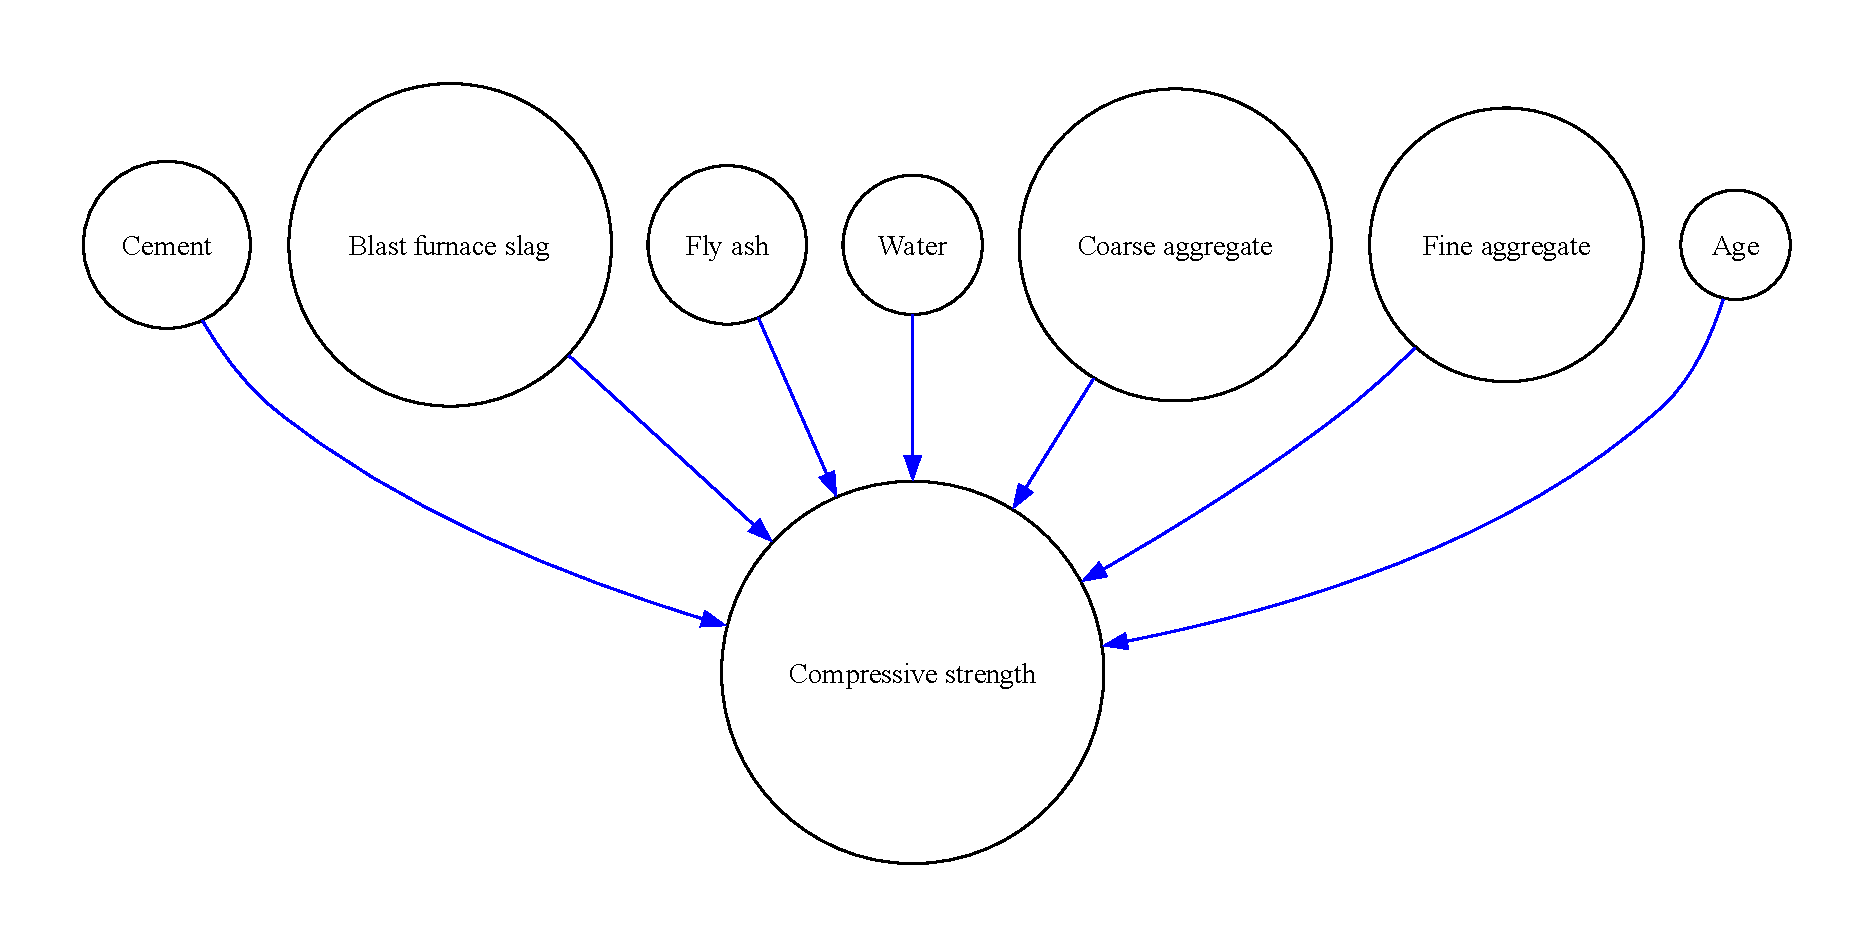
\includegraphics[height=0.4\textheight]{dataset/CCS_Data/output_graph/potential_relation.pdf}}
        \caption{\label{fig:relation}Possible Causal Relation Graph}
    \end{figure}
\end{minipage}


\section{Dataset Descriptions and EDA}
The following is a preview of our original dataset.

\begin{table}[H]
    \centering
    \caption{Dataset Preview}
    
    \resizebox{\textwidth}{!}{
    \begin{tabular}{rrrrrrrrr}
\toprule
 Cement &  Blast furnace slag &  Fly ash &  Water &  Superplasticizer &  Coarse aggregate &  Fine aggregate &  Age &  Compressive strength \\
\midrule
  540.0 &                 0.0 &      0.0 &  162.0 &               2.5 &            1040.0 &           676.0 &   28 &                 79.99 \\
  540.0 &                 0.0 &      0.0 &  162.0 &               2.5 &            1055.0 &           676.0 &   28 &                 61.89 \\
  332.5 &               142.5 &      0.0 &  228.0 &               0.0 &             932.0 &           594.0 &  270 &                 40.27 \\
  332.5 &               142.5 &      0.0 &  228.0 &               0.0 &             932.0 &           594.0 &  365 &                 41.05 \\
  198.6 &               132.4 &      0.0 &  192.0 &               0.0 &             978.4 &           825.5 &  360 &                 44.30 \\
\bottomrule
\end{tabular}
}
                
\end{table}

\subsection{Data Properties}
We employ several statistical methods to identify data properties.

The shape of the data, data types, and missing values are assessed directly from the dataframe.
Linearity is evaluated using Ramsey’s RESET test, followed by the Benjamini \& Yekutieli procedure for multiple test correction.
Gaussian noise is assessed through the Shapiro-Wilk test, also applying the Benjamini \& Yekutieli procedure for multiple test correction.
Time-Series and Heterogeneity are derived from user queries.

Properties of the dataset we analyzed are listed below.

\begin{table}[H]
    \centering
    \caption{Data Properties}

    \begin{tabular}{rrrrrrr}
    \toprule
    Shape ($n$ x $d$) & Data Type & Missing Value & Linearity & Gaussian Errors & Time-Series & Heterogeneity \\
    \midrule
    (1030, 9)   & Continuous & False & False & False & False & False \\
    \bottomrule
    \end{tabular}
        
\end{table}


\subsection{Distribution Analysis}
The following figure shows distributions of different variables. The orange dash line represents the mean, 
and the black line represents the median. Variables are categorized into three types according to their distribution characteristics.

\begin{figure}[H]
\centering
\includegraphics[width=\linewidth]{dataset/CCS_Data/output_graph/eda_dist.jpg}
\caption{\label{fig:dist}Distribution Plots of Variables}
\end{figure}

\begin{itemize}
\item Slight left skew distributed variables: None
\item Slight right skew distributed variables: Blast furnace slag, Fly ash, Age, Compressive strength
\item Symmetric distributed variables: Cement, Water, Superplasticizer, Coarse aggregate, Fine aggregate
\end{itemize}

\subsection{Correlation Analysis}

\begin{minipage}[t]{0.5\linewidth}
    In this analysis, we will categorize the correlation statistics of features in the dataset into three distinct categories: Strong correlations ($r>0.8$), Moderate correlations ($0.5<r<0.8$), and Weak correlations ($r<0.5$).

\begin{itemize}
\item Strong Correlated Variables: None
\item Moderate Correlated Variables: Superplasticizer and Water
\item Weak Correlated Variables: None
\end{itemize}
\vfill
\end{minipage}
\hfill
\begin{minipage}[t]{0.5\linewidth}
    \begin{figure}[H]
        \centering
        \vspace{-1.5cm}
        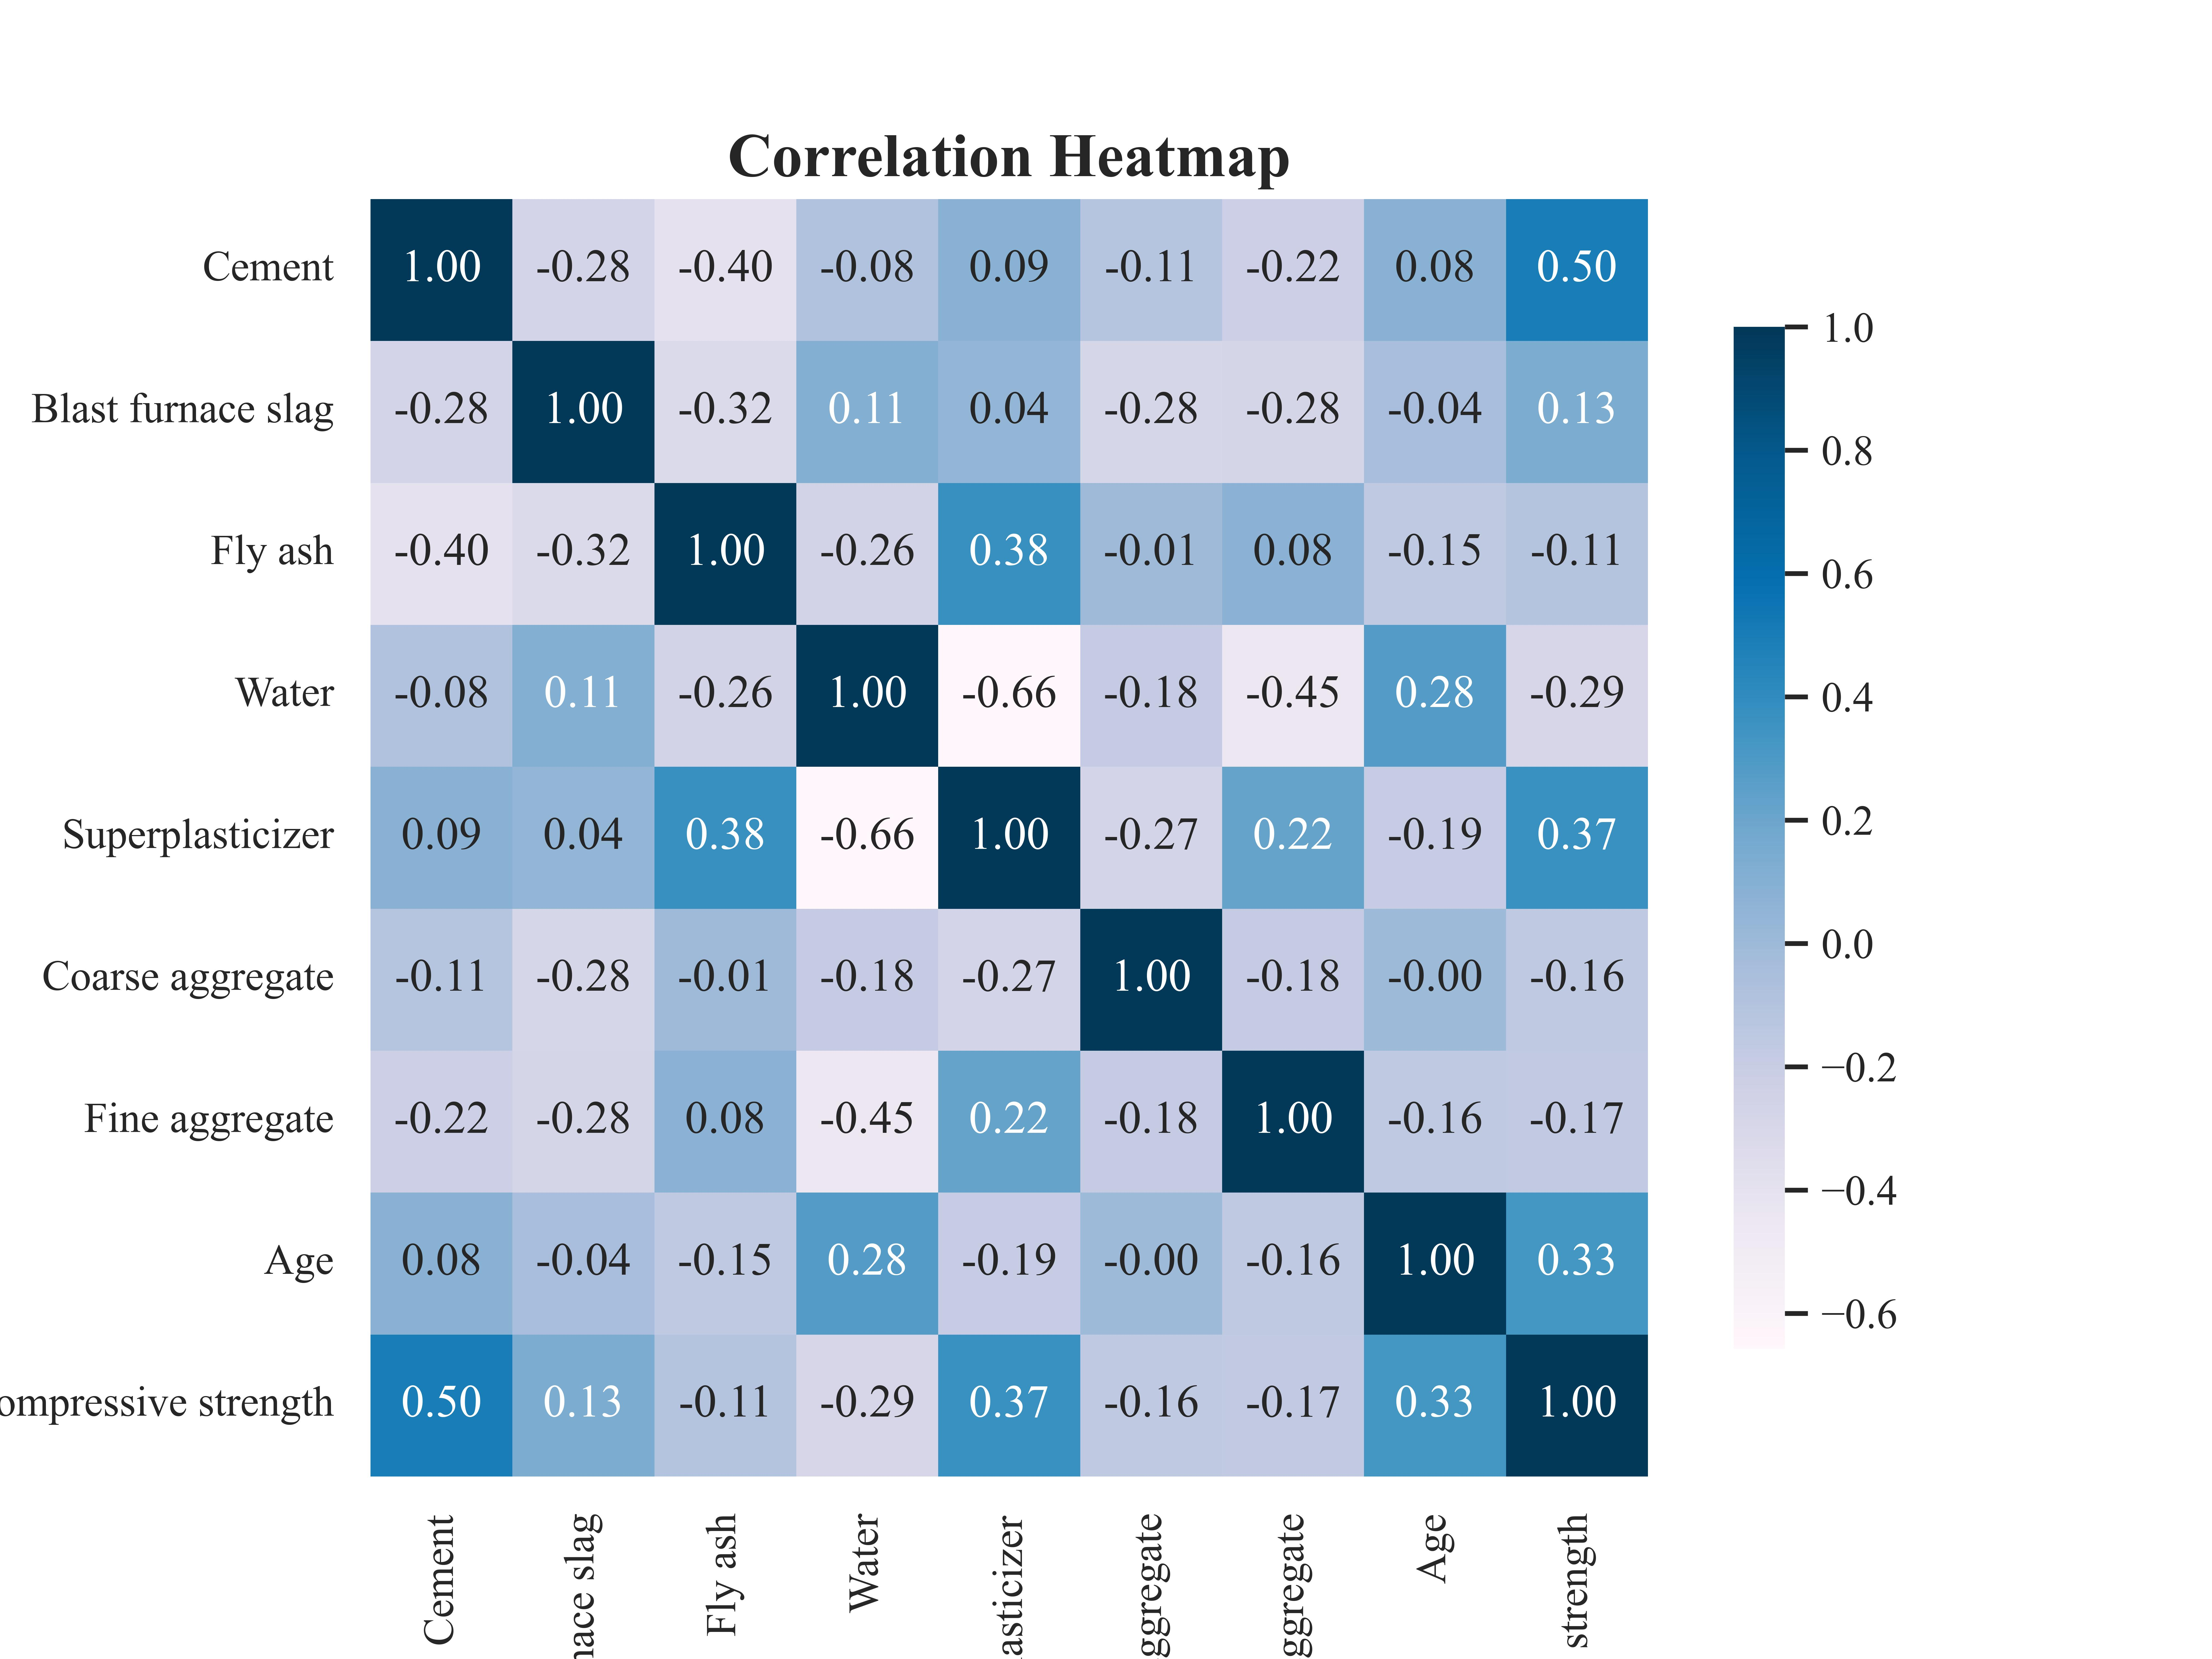
\includegraphics[width=\linewidth]{dataset/CCS_Data/output_graph/eda_corr.jpg}
        \caption{\label{fig:corr}Correlation Heatmap of Variables}
    \end{figure}
\end{minipage}

\section{Discovery Procedure}

In this section, we provide a detailed description of the causal discovery process implemented by Causal Copilot. 
We also provide the chosen algorithms and hyperparameters, along with the justifications for these selections.

\subsection{Data Preprocessing}
In this initial step, we preprocessed the data and examined its statistical characteristics. 
This involved cleaning the data, handling missing values, and performing exploratory data analysis to understand distributions and relationships between variables.
                
\subsection{Algorithm Selection assisted with LLM}
Following data preprocessing, we employed a large language model (LLM) to assist in 
selecting appropriate algorithms for causal discovery based on the statistical characteristics of the dataset and relevant background knowledge. 
The top three chosen algorithms, listed in order of suitability, are as follows:   
        
\begin{itemize}
        
\item \textbf{PC}:
    \begin{itemize}
        \item \textbf{Description}: The PC algorithm is a constraint-based method that learns the structure of a causal graph by testing conditional independencies between variables, resulting in a Directed Acyclic Graph (DAG).
        \item \textbf{Justification}: Given that the dataset has a large sample size (1030) and no missing values, the PC algorithm is suitable as it can efficiently process large datasets. The assumption of causal sufficiency aligns with the absence of hidden confounders, making it a strong first candidate.
    \end{itemize}

\item \textbf{GES}:
    \begin{itemize}
        \item \textbf{Description}: Greedy Equivalence Search (GES) is a score-based algorithm that identifies the optimal causal structure by navigating the space of equivalence classes of Directed Acyclic Graphs (DAGs) using score functions like BIC.
        \item \textbf{Justification}: The GES algorithm is versatile and efficient for large datasets. While it primarily assumes Gaussian distributions, its capability to use generalized scores makes it suitable for this dataset, especially since it allows for a non-Gaussian structure.
    \end{itemize}

\item \textbf{NOTEARS}:
    \begin{itemize}
        \item \textbf{Description}: NOTEARS transforms causal graph learning into a continuous optimization problem, allowing for efficient computation on large datasets while maintaining the acyclicity of the causal structure.
        \item \textbf{Justification}: NOTEARS is recommended because it can handle large datasets and is flexible enough to adapt to nonlinear relationships. Given the evidence that relationships are not predominantly linear, this method could be an effective exploratory tool for capturing more complex relationships.
    \end{itemize}

\end{itemize}
                    

\subsection{Hyperparameter Values Proposal assisted with LLM}
Once the algorithms were selected, the LLM aided in proposing hyperparameters 
for the [ALGO] algorithm, which are specified below:
        
\begin{itemize}

\item \textbf{alpha}:
    \begin{itemize}
        \item \textbf{Value}: 0.01
        \item \textbf{Explanation}: Given the large sample size of 1030, a lower significance level (0.01) is appropriate to reduce the likelihood of false positives when determining conditional independence. This helps to ensure that the discovered edges in the causal graph reflect true relationships.
    \end{itemize}

\item \textbf{indep\_test}:
    \begin{itemize}
        \item \textbf{Value}: fisherz
        \item \textbf{Explanation}: Since the dataset consists of continuous data, 'fisherz' is the suitable choice for the independence test method. It is efficient for continuous datasets; however, caution is advised as the underlying assumptions of linearity and Gaussianity are not met, but it is still the best option given the dataset structure.
    \end{itemize}

\item \textbf{depth}:
    \begin{itemize}
        \item \textbf{Value}: -1
        \item \textbf{Explanation}: The default value of -1 for depth is appropriate as it allows the PC algorithm to explore the entire causal structure without depth restrictions. This is beneficial given the comprehensive nature of the dataset and ensures a complete analysis of potential relationships among variables.
    \end{itemize}

\end{itemize}

        
\subsection{Graph Tuning with LLM Suggestion}
In the final step, we performed graph tuning with suggestions provided by the LLM.
We utilize LLM to help us determine the direction of undirected edges according to its knowledge repository.
By integrating insights from the LLM to refine the causal graph, we can achieve improvements in graph's accuracy and robustness.
            
\item \textbf{Fine aggregate $\rightarrow$ Blast furnace slag}: Fine aggregate is a component of the concrete mix and is influenced by the overall mixture, including the addition of blast furnace slag. Thus, the presence of fine aggregate affects how blast furnace slag operates within the mix.

\item \textbf{Superplasticizer $\rightarrow$ Compressive strength}: Superplasticizers enhance the workability of concrete, allowing for a better mix that can improve the compressive strength, thus indicating that superplasticizers cause an increase in compressive strength.

            
This structured approach ensures a comprehensive and methodical analysis of the causal relationships within the dataset.
        

\section{Results Summary}

\begin{figure}[H]
    \centering
    \begin{subfigure}{0.3\textwidth}
        \centering
        \vspace{-0.5cm}
        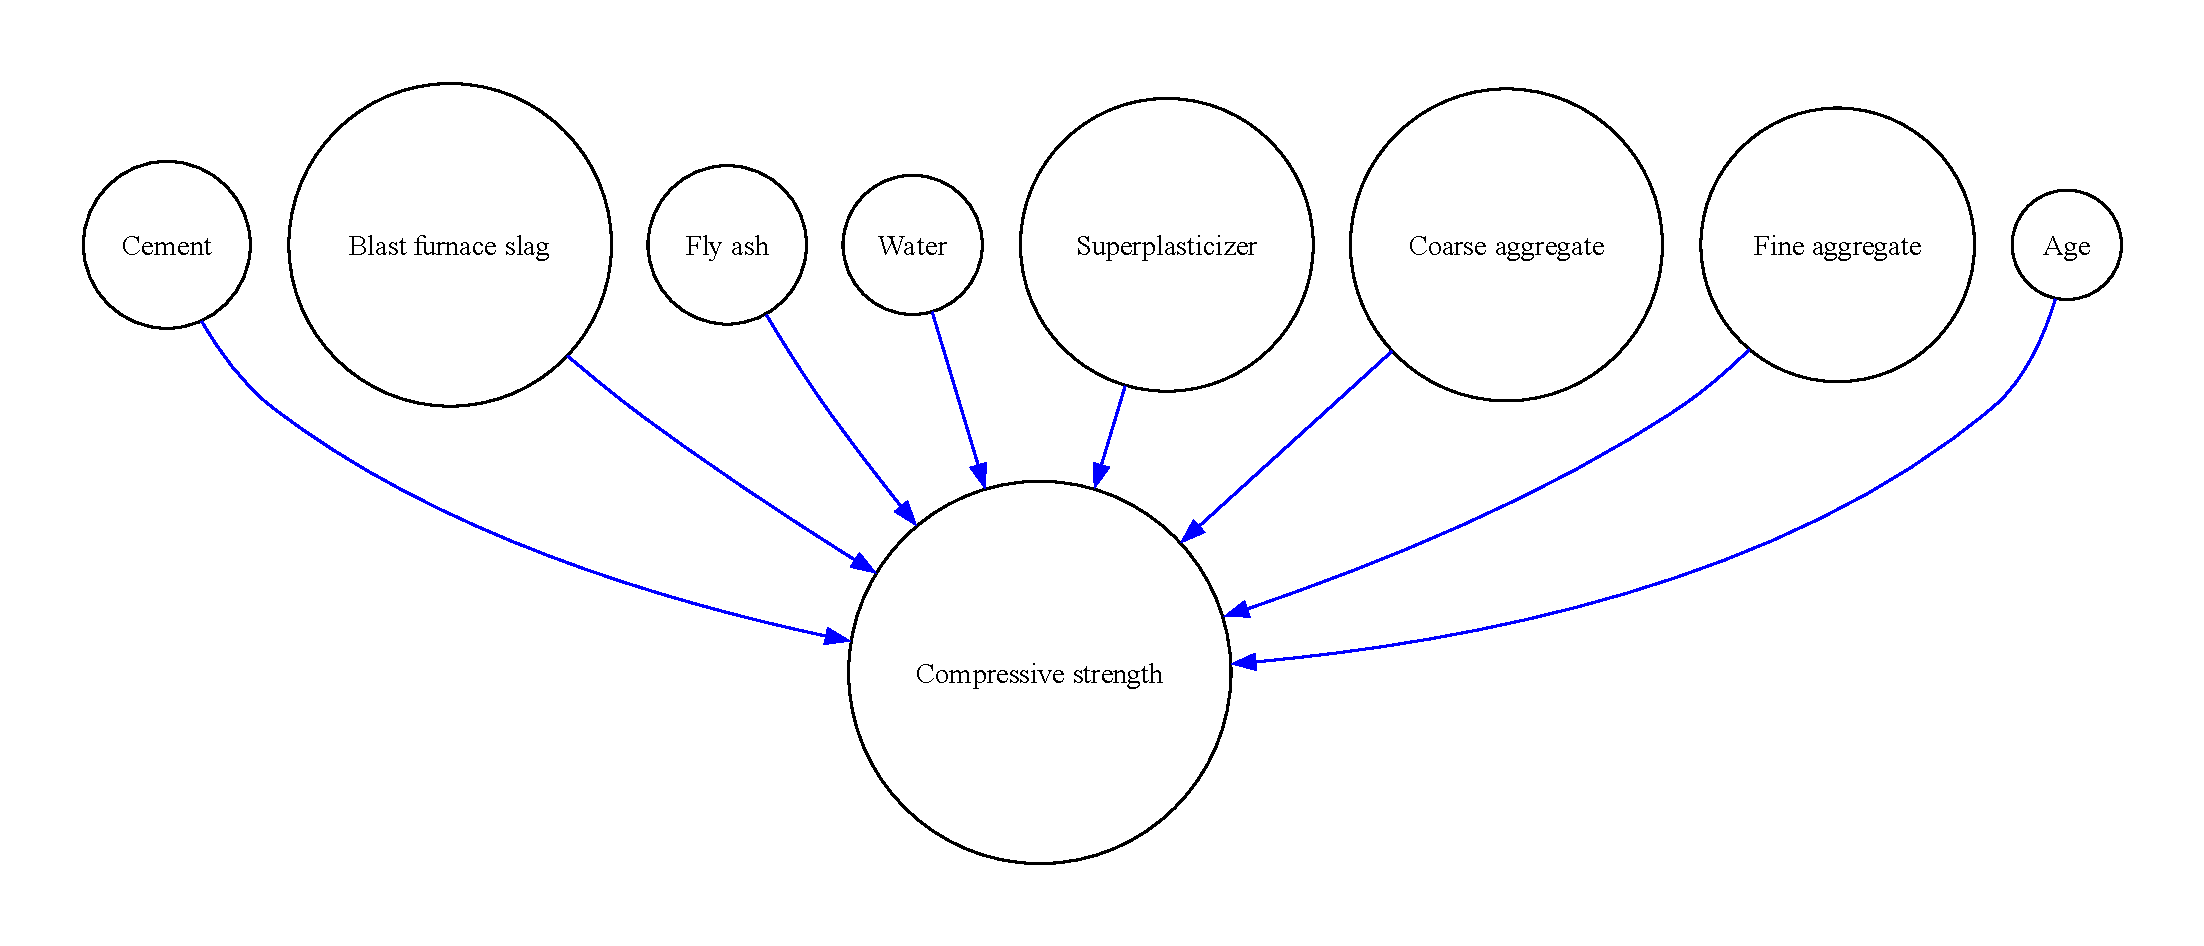
\includegraphics[width=\linewidth]{dataset/CCS_Data/output_graph/true_graph.pdf}
        \vfill
        \caption{True Graph}
        \label{fig:sub1}
    \end{subfigure}
    \hspace{0.04\textwidth}
    \begin{subfigure}{0.3\textwidth}
        \centering
        \vspace{-0.5cm}
        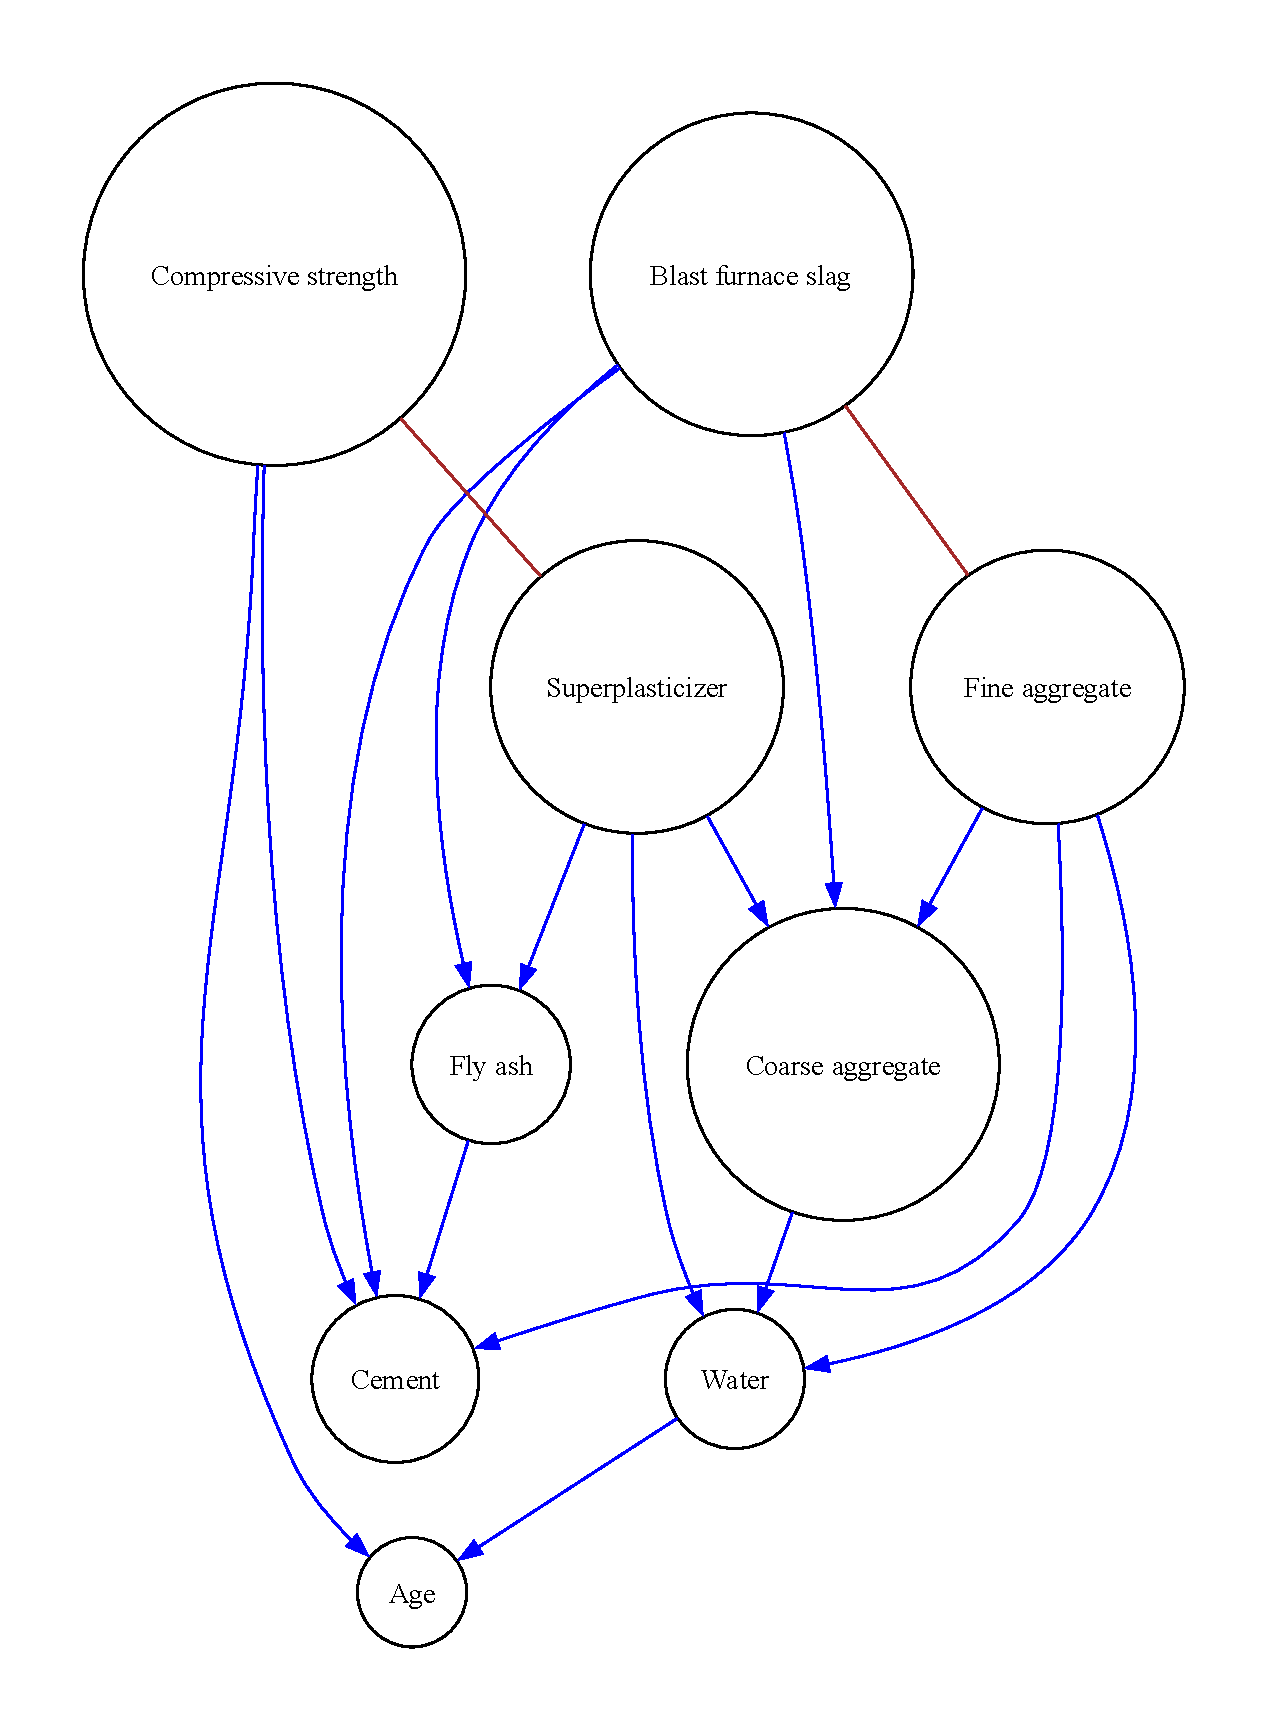
\includegraphics[width=\linewidth]{dataset/CCS_Data/output_graph/initial_graph.pdf}
        \vfill
        \caption{Initial Graph}
        \label{fig:sub2}
    \end{subfigure}
    \hspace{0.04\textwidth}
    \begin{subfigure}{0.3\textwidth}
        \centering
        \vspace{-0.5cm}
        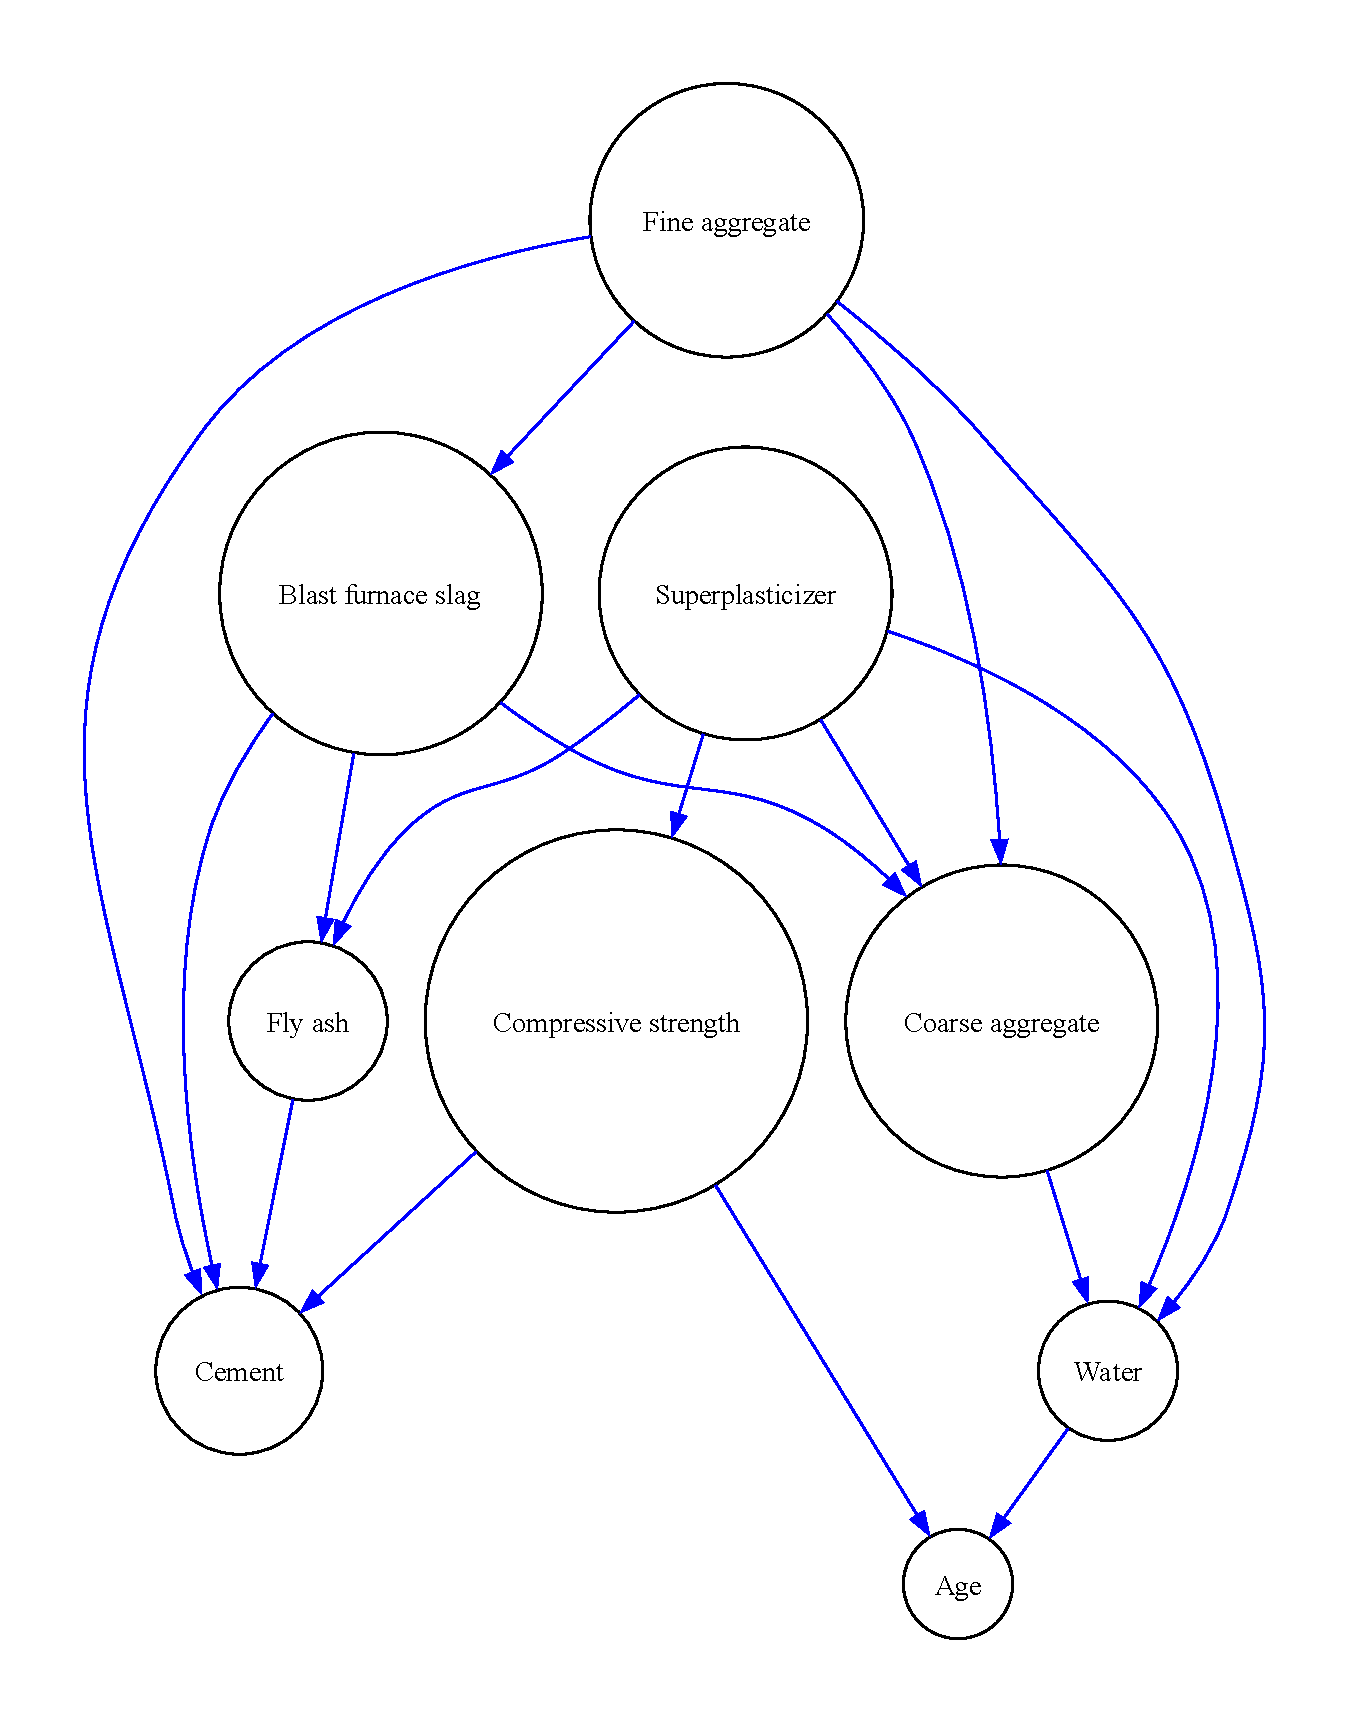
\includegraphics[width=\linewidth]{dataset/CCS_Data/output_graph/revised_graph.pdf}
        \vfill
        \caption{Revised Graph}
        \label{fig:sub3}
    \end{subfigure}
    \caption{Graphs Comparison of PC}
    \label{fig:main}
\end{figure}

The above are result graphs produced by our algorithm.
The initial graph is the graph in the first attempt, and the revised graph is the one pruned with LLM suggestion.

The analysis reveals an intricate web of causal relationships among the various components typically used in concrete production. Blast furnace slag plays a pivotal role, influencing not only Cement but also Fly ash, Coarse aggregate, and Fine aggregate, which are essential for enhancing the properties of concrete. The Fly ash, often utilized as a supplementary cementitious material, is also affected by the presence of Superplasticizer, which further interacts with Water, optimizing the viscosity and workability of the concrete mix. Superplasticizer itself has a significant effect on Coarse aggregate and Compressive strength, a crucial property indicating the concrete's load-bearing capacity. Additionally, Fine aggregate acts as a critical determinant, influencing both Cement and the other aggregates while also being connected to Water, which is vital in the hydration process. Ultimately, the relationship among Compressive strength, Cement, and Age emphasizes how the material's performance develops over time, highlighting the role of each component in achieving the desired durability and strength of the concrete mixture.

\subsection{Graph Reliability Analysis}

\begin{figure}[H]
        \centering
        \vspace{-0.5cm}
        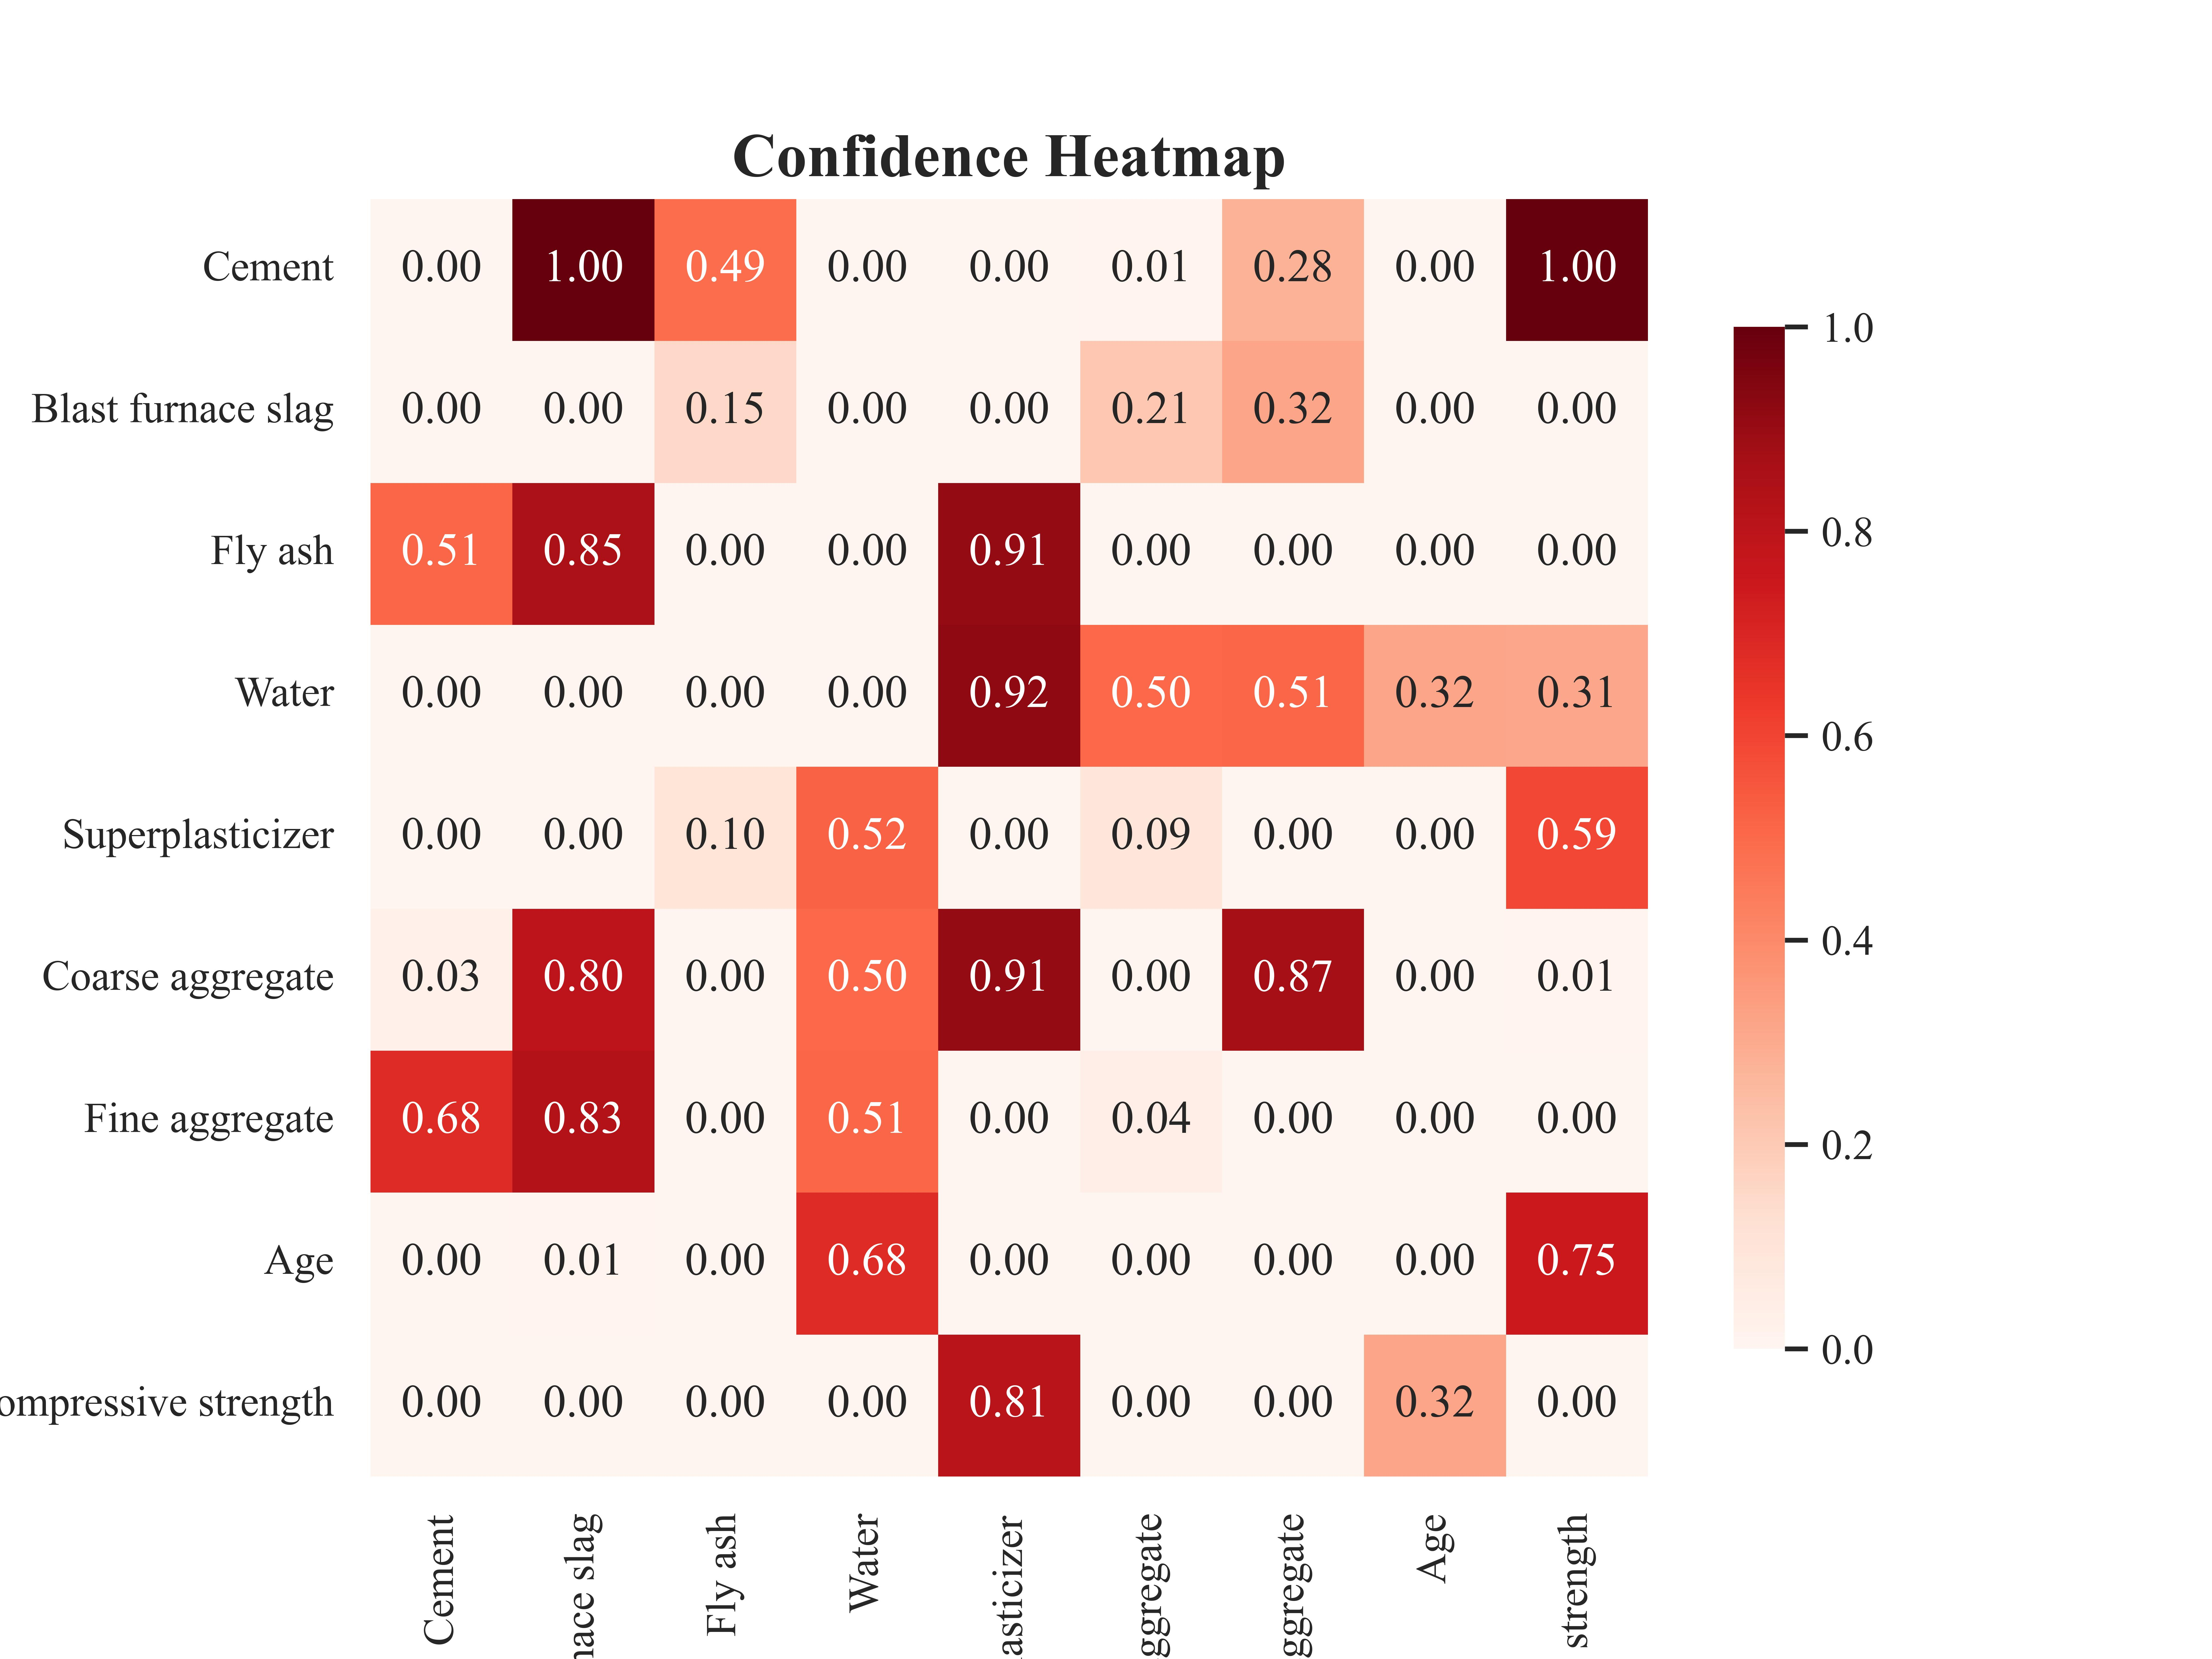
\includegraphics[width=0.8\linewidth]{dataset/CCS_Data/output_graph/confidence_heatmap.jpg}
        \caption{Reliability Graph}
        \label{fig:sub3}
\end{figure}

Based on the confidence probability heatmap and background knowledge, we can analyze the reliability of our graph.

From the statistics perspective, we have high confidence to believe that the edges Fly ash $\rightarrow$ Cement (0.51), Water $\rightarrow$ Age (0.32), Superplasticizer $\rightarrow$ Water (0.52), Superplasticizer $\rightarrow$ Compressive strength (0.59), Fine aggregate $\rightarrow$ Cement (0.68), Fine aggregate $\rightarrow$ Blast furnace slag (0.83), and Compressive strength $\rightarrow$ Superplasticizer (0.81) exist due to their sufficiently high bootstrap probabilities. Conversely, we have low confidence in the edges Blast furnace slag $\rightarrow$ Cement (0.0), Compressive strength $\rightarrow$ Cement (0.0), and Superplasticizer $\rightarrow$ Coarse aggregate (0.09), indicating these edges likely do not exist.

However, based on expert knowledge, we know that the connection between Cement and Compressive strength is a well-established relationship in concrete science; cement quantity significantly influences compressive strength, which contradicts the statistical edge reliability given (0.0). Additionally, while the edge between Fly ash and Cement is statistically supported (0.51), expert knowledge informs us that Fly ash typically acts as a pozzolanic material rather than directly causing changes in the cement amount used.

Therefore, the result of this causal graph is not entirely reliable, as discrepancies exist between the statistical evidence and established domain knowledge in concrete science, particularly regarding critical relationships like Cement $\rightarrow$ Compressive strength and Fly ash $\rightarrow$ Cement.

\end{document}